\section{APIs}
\label{api}

Eine API ermöglicht es, dass unabhängige Anwendungen miteinander kommunizieren und Daten austauschen können~\cite{api}.
Im Allgemeinen funktioniert diese Kommunikation mit dem HTTP-Protokoll über das Internet~\cite[vgl.]{awsrestgraphql}.
Dabei stellt ein System per HTTP eine Anfrage und die API liefert eine Antwort.
Es ist nicht festgelegt, auf welche Art das System die Antwort für die API erzeugt.
Dies hängt stark von der zugrundeliegenden Implementierung ab.

\begin{figure}[h!]
    \centering
    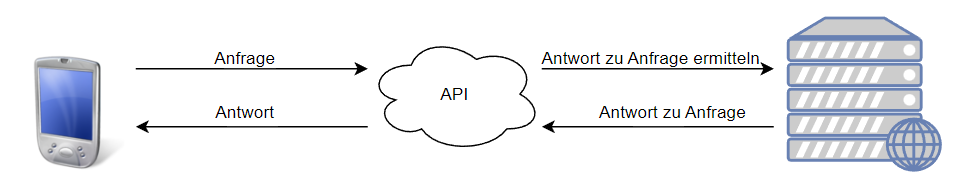
\includegraphics[width=\textwidth,height=\textheight,keepaspectratio]{img/webapi}
    \caption{simple API-Kommunikation}
    \label{basicapi}
\end{figure}

Es gibt verschiedene Entwurfsmuster, die für ein API Design genutzt werden können.
Die verschiedenen Muster werden durch Programmcode umgesetzt und sind somit fehleranfällig.

\newpage